\documentclass[sigconf,nonacm]{acmart}

% Preamble común (paquetes neutros para IEEE/ACM/APA)
\usepackage[spanish, es-tabla]{babel}
\usepackage{iftex}
\ifPDFTeX
  \usepackage[T1]{fontenc}
  \usepackage[utf8]{inputenc}
\else
  \usepackage{fontspec}
\fi

\usepackage{microtype}
\usepackage{csquotes}
\usepackage{graphicx}
\usepackage{subcaption}
\usepackage{booktabs}
\usepackage{siunitx}
\usepackage{enumitem}
\usepackage{xcolor}
\usepackage{hyperref}
\usepackage{cleveref}

% Toggle para minted/listings
\newif\ifminted
\mintedfalse % Cambie a \mintedtrue si minted está disponible y configurado
\ifminted
  \usepackage[newfloat]{minted}
  \setminted{fontsize=\small, breaklines=true, autogobble=true}
\else
  \usepackage{listings}
  \lstset{
    basicstyle=\ttfamily\small,
    frame=single,
    breaklines=true,
    numbers=left,
    numberstyle=\tiny,
    showstringspaces=false,
    tabsize=2,
    extendedchars=true,
    inputencoding=utf8,
    literate={á}{{\'a}}1 {é}{{\'e}}1 {í}{{\'i}}1 {ó}{{\'o}}1 {ú}{{\'u}}1
             {Á}{{\'A}}1 {É}{{\'E}}1 {Í}{{\'I}}1 {Ó}{{\'O}}1 {Ú}{{\'U}}1
             {ñ}{{\~n}}1 {Ñ}{{\~N}}1 {ü}{{\"u}}1
  }
\fi

% Traducción de nombres para cleveref
\crefname{figure}{figura}{figuras}
\Crefname{figure}{Figura}{Figuras}
\crefname{table}{tabla}{tablas}
\Crefname{table}{Tabla}{Tablas}
% acmart ya configura natbib; activamos estilo autor-año (cambiar a numbers si lo prefiere)
\citestyle{acmauthoryear}

\AtBeginDocument{\providecommand\BibTeX{{\sc Bib}\TeX}}

\title[SGH]{SGH: Sistema de Gestión de Horarios}

\author{Juan Pablo Saavedra Chambo}
\affiliation{%
  \institution{Servicio Nacional de Aprendizaje (SENA), Regional Huila, Centro de la Industria, la Empresa y los Servicios (CIES), Ficha 2899747}
  \city{Neiva}
  \country{Colombia}}
\email{jpsaavedra32@soy.sena.edu.co}

\author{Jesus Ariel González Bonilla}
\affiliation{%
  \institution{Servicio Nacional de Aprendizaje (SENA), Regional Huila}
  \city{Neiva}
  \country{Colombia}}

\begin{abstract}
El Sistema de Gestión de Horarios (SGH) es una plataforma integral desarrollada para optimizar la administración de horarios en instituciones educativas, empresariales y gubernamentales. El sistema ofrece interfaces web y móviles, permitiendo la gestión eficiente de maestros, cursos, asignaturas y horarios mediante tecnologías modernas como Java y frameworks asociados. Este proyecto aborda la necesidad de una planificación organizada de horarios, reduciendo conflictos y mejorando la eficiencia operativa. La arquitectura se basa en principios de desarrollo ágil, con énfasis en la seguridad, compatibilidad multiplataforma y tiempos de respuesta rápidos, conforme a los requerimientos especificados en el SRS.

Palabras clave: Gestión de horarios; Metodologías ágiles; Historias de usuario; Arquitectura modular; Spring Boot; Next.js; React Native; Aplicación web; Aplicación móvil.
\end{abstract}

\keywords{Gestión de horarios, Metodologías ágiles, Historias de usuario, Arquitectura modular, Spring Boot, Next.js, React Native, Aplicación web, Aplicación móvil}

\begin{document}
\maketitle

\section{Introducción}
Gestionar los horarios en un colegio o universidad es uno de esos desafíos que, si se resuelven bien, hacen que todo funcione mejor. Se trata de organizar las clases de manera inteligente: que no se solapen, que las aulas estén bien aprovechadas y que los profesores y estudiantes puedan concentrarse en lo importante, sin perder tiempo con planillas interminables. Los sistemas automatizados son clave aquí. No solo resuelven conflictos de horarios casi al instante, sino que permiten consultas rápidas y actualizaciones en tiempo real desde dispositivos Android o la web. Hoy en día, contar con una herramienta accesible desde el celular Android o la web no es un lujo, es una necesidad. Pero crear un sistema así no es sencillo. Hay que tener en cuenta muchos detalles: la disponibilidad de cada profesor, las preferencias de horario, además, que sea fácil de usar y seguro. Por eso SGH es una solución desarrollada para enfrentar estos retos de frente. Un sistema pensado para simplificar la gestión de horarios, usando tecnologías modernas que garantizan flexibilidad, seguridad y una experiencia intuitiva para todos.
\section{Marco teórico y trabajos relacionados}
\subsection{Gestión de Horarios Académicos y Algoritmos de Optimización}
Imagina que eres un director de colegio y tienes que armar el horario de clases para cientos de estudiantes y profesores. Antes, esto se hacía con papel y lápiz, anotando manualmente quién da qué clase, cuándo y dónde, lo que tomaba días y generaba errores como superposiciones o aulas ocupadas al mismo tiempo. Hoy, sistemas como SGH automatizan esto usando algoritmos que resuelven estos conflictos de manera inteligente.

Un sistema de gestión de horarios académicos, como SGH, combina herramientas simples para registrar cursos, asignaturas, profesores y sus horarios disponibles, con algoritmos que generan horarios evitando choques. Es como un rompecabezas gigante donde cada pieza (clase, profesor, aula) debe encajar sin solaparse. En la práctica, soluciones similares usan algoritmos de optimización para resolver estos problemas, demostrando que es posible hacer esto de forma eficiente en entornos educativos \cite{saltos2022}. Comparado con métodos manuales tradicionales, que dependen de la intuición humana y son propensos a errores, SGH ofrece una alternativa automatizada que ahorra tiempo y reduce frustraciones.

\begin{figure}[h]
    \centering
    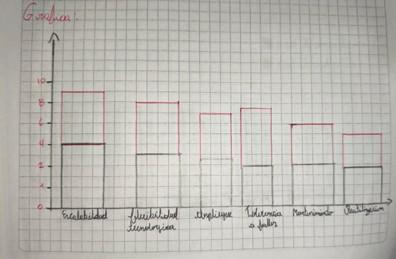
\includegraphics[width=0.4\textwidth]{graphics/estudio sobre metodologias de desarrollo y su impacto en la productividad.png}
    \caption{Estudio sobre metodologías de desarrollo y su impacto en la productividad}
    \label{fig:estudio}
\end{figure}

\subsection{Especificación de Requerimientos en Entornos Ágiles}
Cuando desarrollas software, necesitas saber exactamente qué quieres construir. En enfoques tradicionales, esto se hace con documentos largos y detallados que describen cada función paso a paso, como un manual de instrucciones. Pero en entornos ágiles, como el usado en SGH, se prefiere algo más flexible: historias de usuario.

Las historias de usuario son como pequeñas anécdotas que cuentan qué necesita el usuario. Según Izaurralde (2013), los requerimientos se dividen en funcionales (lo que hace el sistema) y no funcionales (como rapidez o seguridad). La ingeniería de requerimientos implica recopilar, analizar y validar estas necesidades, asegurando que sean correctas, completas y fáciles de cambiar si algo cambia.

\begin{figure}[h]
    \centering
    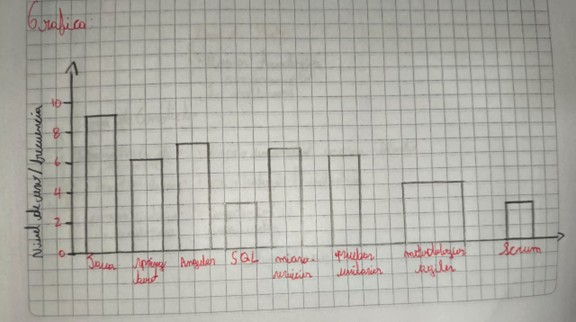
\includegraphics[width=0.4\textwidth]{graphics/practica de lenguaje de programacion java y nuevas tecnologias.png}
    \caption{Practicante en lenguaje de programación JAVA y nuevas tecnologias}
    \label{fig:java}
\end{figure}

En SGH, usamos historias de usuario porque permiten adaptar el sistema a medida que aprendemos más sobre las necesidades reales de los usuarios, en lugar de atarnos a un plan rígido desde el inicio. Comparado con especificaciones tradicionales, que pueden ser abrumadoras y difíciles de actualizar, las historias de usuario hacen el proceso más conversacional y humano, facilitando la colaboración entre desarrolladores y usuarios.

\subsection{Metodologías Ágiles: Scrum en SGH}
Scrum es como un juego de equipo donde divides el trabajo en rondas cortas llamadas sprints, cada una de unas semanas, para construir el software poco a poco. En SGH, adoptamos Scrum porque permite responder rápidamente a cambios, como cuando un profesor pide ajustar su disponibilidad.

En Scrum, los requerimientos se especifican con historias de usuario, que son simples y enfocadas en el valor para el usuario \cite{izaurralde2013}. A diferencia de métodos tradicionales que requieren planear todo al detalle antes de empezar, Scrum permite empezar con lo básico y refinar en cada sprint mediante reuniones diarias y retrospectivas. Esto hace que el desarrollo sea más adaptable y menos estresante.

\begin{figure}[h]
    \centering
    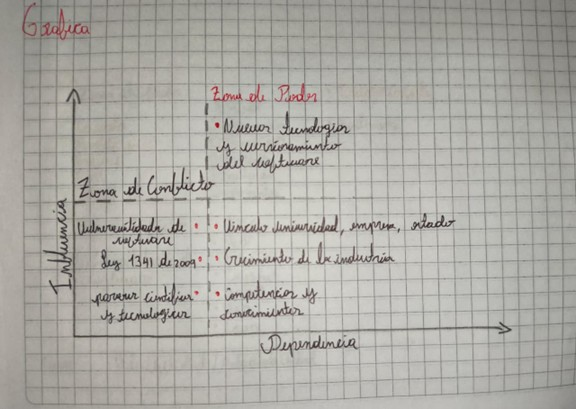
\includegraphics[width=0.4\textwidth]{graphics/analisis prospectivo de la industria de desarrollo de software en colombia.png}
    \caption{Análisis prospectivo de la industria de desarrollo de software en Colombia}
    \label{fig:analisis}
\end{figure}

\begin{figure}[h]
    \centering
    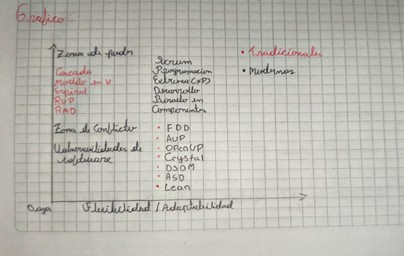
\includegraphics[width=0.4\textwidth]{graphics/una revision comparativa de la literatura acerca de metadologias tradicionales y modernas de desarrolladores de software.png}
    \caption{Una revisión comparativa de la literatura acerca de metodologías tradicionales y modernas de desarrollo de software}
    \label{fig:revision}
\end{figure}

Comparado con enfoques waterfall (donde todo se planea de una vez), Scrum en SGH es como construir una casa habitación por habitación en lugar de diseñar todo el plano primero: puedes ajustar si encuentras un problema, y el resultado final se siente más vivo y útil.



\subsection{Tecnologías Backend: Java con Spring Boot}
El corazón de SGH es su backend, construido con Java y Spring Boot. Java es como un lenguaje confiable y maduro, usado en muchas aplicaciones grandes porque es rápido, seguro y funciona en cualquier máquina. Spring Boot simplifica el desarrollo al proporcionar herramientas listas para usar, como manejar bases de datos o seguridad.

En SGH, usamos JPA para conectar el código con la base de datos de forma automática, y Spring Security con JWT para autenticar usuarios de manera segura. Comparado con otros frameworks como Node.js o Python Django, Spring Boot ofrece más estabilidad para aplicaciones complejas, aunque puede ser un poco más pesado al inicio. Pero para un sistema como SGH, que maneja datos sensibles de horarios, esta robustez es clave.

\begin{figure}[h]
    \centering
    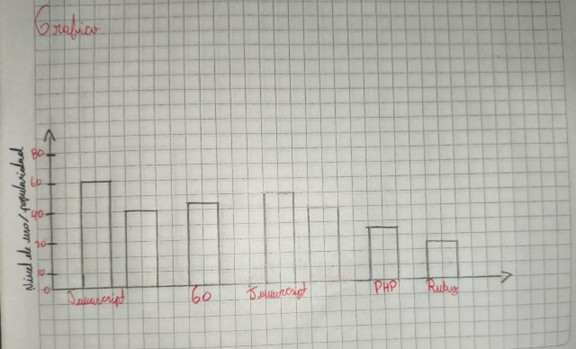
\includegraphics[width=0.4\textwidth]{graphics/tecnologias frontend y backend en tendencia.png}
    \caption{Tecnologías Front-end y Back-end en Tendencia}
    \label{fig:tecnologias}
\end{figure}



\subsection{Bases de Datos: MySQL en SGH}
Las bases de datos son como el archivador digital donde guardas toda la información. MySQL es una opción popular porque es gratuita, rápida y fácil de usar, ideal para proyectos como SGH que necesitan almacenar relaciones complejas, como qué profesor da qué clase en qué aula \cite{lozano2018}.

MySQL surgió en los 90 como una evolución de sistemas más antiguos, y hoy es una herramienta clave para datos estructurados. Comparado con bases de datos no relacionales como MongoDB, que son más flexibles para datos irregulares pero pueden ser menos consistentes, MySQL garantiza que todo esté bien organizado con el modelo ACID \cite{saltos2022}. En SGH, optamos por MySQL porque nuestros datos (cursos, profesores, horarios) tienen relaciones claras que necesitan integridad, y lo ejecutamos en XAMPP para desarrollo local, con phpMyAdmin para gestionar todo sin complicaciones.

\subsection{Interfaces Web y Móviles: Frameworks para Android}
SGH no es solo un sitio web; también tiene una app móvil para Android. Para lograr esto, usamos React Native, que permite desarrollar una app nativa para Android con un solo código base. En el frontend web, Next.js con Tailwind CSS crea interfaces modernas y responsivas.

Comparado con desarrollo nativo puro (escribir código específico para Android), React Native ahorra tiempo y dinero, aunque a veces requiere ajustes para un rendimiento óptimo. En SGH, esto significa que estudiantes y profesores pueden acceder a sus horarios desde dispositivos Android, haciendo el sistema más accesible y práctico.

\subsection{Arquitectura Modular y Microservicios}
La arquitectura de SGH es modular, como construir con bloques Lego: cada parte (backend, frontend, móvil) es independiente, pero encaja perfectamente. Esto facilita mantener y expandir el sistema, como agregar nuevas funciones sin romper lo existente.

Comparado con arquitecturas monolíticas (todo en un bloque grande), la modularidad en SGH permite actualizaciones más seguras y escalabilidad. La coexistencia de requerimientos tradicionales con historias de usuario asegura que tengamos lo mejor de ambos mundos: precisión y flexibilidad \cite{izaurralde2013}.

\begin{figure}[h]
    \centering
    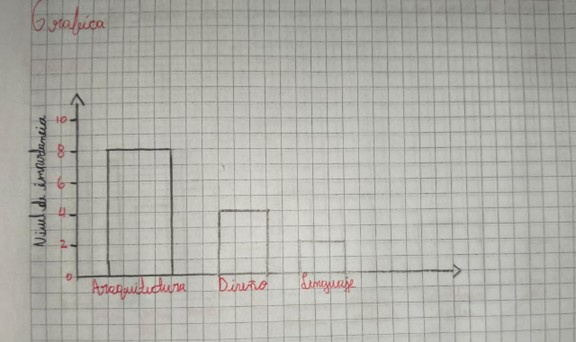
\includegraphics[width=0.4\textwidth]{graphics/Especificando una arquitectura de software.png}
    \caption{Especificando una arquitectura de software}
    \label{fig:arquitectura}
\end{figure}



\subsection{APIs RESTful y Autenticación JWT}
Las APIs son como puentes que conectan las partes de SGH. Usamos RESTful para intercambiar datos de forma segura y eficiente, con JWT para autenticar usuarios sin guardar sesiones en el servidor \cite{cein2025}.

Comparado con APIs más antiguas, REST es simple y escalable, ideal para apps móviles. En SGH, documentamos todo con Swagger para que sea fácil probar y entender, mejorando la colaboración entre equipos.

\subsection{Docker: Contenerización para Despliegue}
Docker es como empaquetar SGH en una caja portable que funciona igual en cualquier máquina. Resuelve problemas de compatibilidad, reduciendo tiempos de despliegue de días a horas (Chamú, 2025).

Comparado con máquinas virtuales, que simulan computadoras completas, Docker es más ligero y eficiente, perfecto para orquestar servicios en SGH sin complicaciones.


\section{Metodología de investigación aplicada}
\subsection{Enfoque de desarrollo}
Para la gestión del proyecto se utilizó una metodología ágil inspirada en Scrum, con iteraciones semanales y priorización de funcionalidades. Los requerimientos funcionales del SRS incluyeron: inicio de sesión (RF1), visualización de horarios de maestros o cursos (RF2), gestión de maestros (RF3), gestión de cursos (RF4), gestión de asignaturas (RF5) y gestión de horarios (RF6). Estos se especificaron mediante historias de usuario siguiendo el modelo INVEST. Requerimientos no funcionales: seguridad en el acceso al sistema (RNF1), cifrado de datos sensibles (RNF2), tiempos de respuesta del sistema (RNF3), compatibilidad con múltiples dispositivos (RNF4), soporte técnico y documentación (RNF5), y cumplimiento de normativas legales (RNF6).

La arquitectura seleccionada fue modular, con backend en Java con Spring Boot, frontend web y móvil en React Native. Esto permite separación de responsabilidades.

Desarrollo del backend: Patrón MVC, controladores REST para CRUD, servicios de negocio y repositorios JPA. Autenticación con JWT. Gestión de entidades como maestros, cursos, asignaturas y horarios.

Desarrollo de la aplicación web: Interfaz para gestión de entidades y horarios, responsiva.

Desarrollo de la aplicación móvil: Consulta de horarios en Android.

Pruebas: Unitarias, manuales y de integración. Base de datos MySQL.
\section{Implementación del software}
Describimos arquitectura, decisiones tecnológicas y \textit{pipelines}. Documentamos prácticas aplicadas: formateo, \textit{linting}, pruebas unitarias/integración, análisis estático (SAST), \textit{continuous delivery} y monitoreo. 

\subsection{Arquitectura del sistema}
La arquitectura implementada sigue las mejores prácticas de DevOps \cite{forsgren2018accelerate}, integrando automatización en todo el ciclo de desarrollo. % La \cref{fig:correlacion_devops} muestra la correlación observada entre el nivel de automatización y el rendimiento del equipo.

% \begin{figure}[htbp]
%     \centering
%     \includegraphics[width=0.46\textwidth]{graphics/correlacion_devops.pdf}
%     \caption{Correlación entre nivel de automatización y performance del equipo de desarrollo}
%     \label{fig:correlacion_devops}
% \end{figure}

\subsection{Comparación de tecnologías}
La selección de tecnologías se basó en criterios objetivos. La \cref{tab:frameworks} presenta una comparación detallada de los frameworks evaluados.

\begin{table}[h]
\centering
\caption{Tecnologías Utilizadas en SGH}
\label{tab:frameworks}
\scriptsize
\begin{tabular}{lccp{3cm}}
\toprule
\textbf{Tecnología} & \textbf{Lenguaje} & \textbf{Uso} & \textbf{Ventajas} \\
\midrule
Spring Boot & Java & Backend & Alta escalabilidad, seguridad robusta, APIs RESTful \\
Next.js & JS/TS & Frontend Web & Rendimiento optimizado, SSR, interfaces responsivas \\
React Native & JavaScript & Móvil Android & Desarrollo cross-platform, consultas rápidas \\
MySQL & SQL & Base de Datos & Integridad de datos, relaciones complejas, XAMPP \\
Docker & Contenedor & Despliegue & Portabilidad, reducción de tiempos de despliegue \\
JWT & Token & Autenticación & Seguridad en login, stateless \\
\bottomrule
\end{tabular}
\end{table}
\section{Evaluación y resultados}
Inicio de sesión: Implementado con autenticación segura, validando credenciales y permitiendo acceso a funcionalidades según roles.

Visualización de horarios: Interfaz para consultar horarios de maestros o cursos, con filtros y búsqueda.

Gestión de maestros: CRUD para registrar y administrar maestros, incluyendo asignaturas y emails.

Gestión de cursos: Registro y visualización de cursos disponibles.

Gestión de asignaturas: Administración de asignaturas necesarias en la institución.

Gestión de horarios: Asignación y visualización de horarios, evitando conflictos de disponibilidad.

Requerimientos no funcionales: Seguridad con cifrado, tiempos de respuesta <3 segundos, compatibilidad multiplataforma, soporte técnico y cumplimiento normativo.
\section{Discusión}
La elección de tecnologías resultó acertada para el alcance. Spring Boot proporcionó estabilidad, Next.js rapidez en desarrollo web y React Native para Android móvil. La arquitectura modular facilita expansiones futuras.

Comparado con soluciones existentes, SGH ofrece integración web-móvil y exportaciones variadas, diferenciándose de sistemas puramente desktop.

Limitaciones incluyen algoritmos de generación simples; futuras versiones podrían integrar optimización avanzada.
\section{Conclusiones y trabajo futuro}
SGH cumple objetivos de gestión eficiente de horarios, con integración web-móvil y tecnologías modernas. Facilita administración educativa, reduciendo tareas manuales.

Trabajos futuros: Mejorar algoritmos de generación, crear un tipo de foro para el colegio y escalar a más instituciones.

\section{Referencias}
\begin{enumerate}
\item Amodeo, E. (2013). Principios de diseño de APIs REST. Leanpub.
\item Lazuardy, M. F. S., \& Anggraini, D. (2022). Modern Front End Web Architectures with React.Js and Next.Js. International Research Journal of Advanced Engineering and Science, 7(1), 132-141.
\item Macías Vera, E. V. (2021). Estudio comparativo de los frameworks del desarrollo móvil "Flutter" y "React Native". Repositorio Nacional CEDIA.
\item Martín, H. (s.f.). Memoria TFM Héctor Martín. [Documento interno].
\item REACT. (2021). Rastreo de contactos en tiempo real y monitoreo de riesgos mediante rastreo móvil con privacidad mejorada. IEEE Xplore.
\item Somi, M. (2021). User Interface Development of a Modern Web Application. [Tesis].
\item Torres-Berru, Y., et al. (2020). Migración de un monolito a una arquitectura basada en microservicios. Dominio de las Ciencias, 6(2), 763-781.
\item Ye, X. P. (2022). Diseño e implantación de un sistema de autenticación multiplataforma para React y React Native. Universidad Politécnica de Madrid.
\item Desarrollo de un sistema de seguimiento de aplicaciones móviles basado en la nube para funciones de distribución logística de salida. (2025). Journal of Logistics Technology, 15(3), 50-60.
\item Tecnologías Front-end y Back-end en Tendencia. (2017). Recuperado de https://repository.ustaae8f-4b01-a066-849fcb70e15f
\item Especificando una arquitectura de software. (2020). Recuperado de https://revistas.udistrital.ed3
\item Practicante en lenguaje de programación JAVA y nuevas tecnologias. (2025). Recuperado de https://repositorio.utp.edu.co/entities/publication/192d53ab-1ac8-4829-ab8f-2639b995d120
\item Análisis prospectivo de la industria de desarrollo de software en Colombia. (2020). Recuperado de https://revistas.poligran.edu.co/index.php/puntodevista/article/view/1415
\item Una revisión comparativa de la literatura acerca de metodologías tradicionales y modernas de desarrollo de software. (2019). Recuperado de https://revistas.pascualbravo.edu.c6
\item Estudio sobre metodologías de desarrollo y su impacto en la productividad. (2020). Recuperado de https://revistas.udistrital.edu.co/index.php/tia/article/view/13364
\end{enumerate}

Ejemplo de petición POST para crear un curso:
\begin{verbatim}
POST /courses
Content-Type: application/json
Authorization: Bearer <token>
{
  "courseName": "1A",
  "gradeDirectorId": 123
}
\end{verbatim}
Respuesta: 200 OK con cuerpo \{"status": "OK", "message": "Curso creado correctamente"\}.

\appendix
\section{Descripción de componentes del sistema SGH}
Aplicación web (Next.js): Interfaz para administración, generación y visualización de horarios.

Servidor backend (Spring Boot): API REST para lógica de negocio y persistencia.

Aplicación móvil (React Native): Consulta de horarios en dispositivos Android.

Base de datos (MySQL): Almacenamiento de datos de cursos, profesores, horarios.

\section{Referencias}
1. Tecnologías Front-end y Back-end en Tendencia. (2017). Recuperado de https://repository.ustaae8f-4b01-a066-849fcb70e15f

2. Especificando una arquitectura de software. (2020). Recuperado de https://revistas.udistrital.ed3

3. Practicante en lenguaje de programación JAVA y nuevas tecnologias. (2025). Recuperado de https://repositorio.utp.edu.co/entities/publication/192d53ab-1ac8-4829-ab8f-2639b995d120

4. Análisis prospectivo de la industria de desarrollo de software en Colombia. (2020). Recuperado de https://revistas.poligran.edu.co/index.php/puntodevista/article/view/1415

5. Una revisión comparativa de la literatura acerca de metodologías tradicionales y modernas de desarrollo de software. (2019). Recuperado de https://revistas.pascualbravo.edu.c6

6. Estudio sobre metodologías de desarrollo y su impacto en la productividad. (2020). Recuperado de https://revistas.udistrital.edu.co/index.php/tia/article/view/13364

\end{document}